\chapter{Literature Review}

Overall methods for robot manipulation can be classified into traditional and data driven methods. Traditional methods are rule based and can be applied for structured and deterministic environments. For stochastic and unstructured environments, data driven methods are used. In this literature review, we will focus of main data driven robot manipulation methods

\section{Reinforcement learning methods}
\begin{figure}[H]
	\centering
	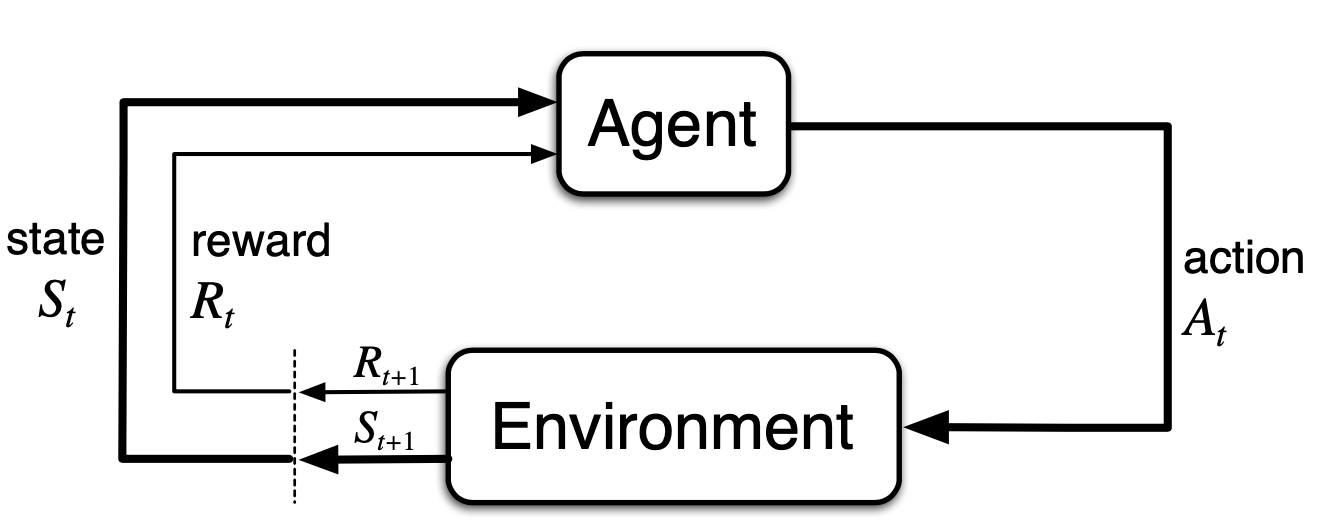
\includegraphics[scale=0.5]{mdp}
	\caption{Reinforcement Learning; Source: \cite{sutton}}
\end{figure}

In reinforcement learning, an agent learns to take actions (policy) based on measured environment state by interacting with the environment through trial and error for maximising a feedback signal (reward or value function). The main challenge in this method is requirement of large amount of data for agent to learn. Collecting large amount of data from real robot will be slow and expensive and might require manual intervention. Instead, for faster and cheaper development, agent can be trained on simulated robot manipulation environment. However policies trained on simulated environments are not directly transferable to real robots due to various differences between simulation and real environments.

\subsection{Comparing Task Simplifications to Learn Closed-Loop Object Picking}
Work done by Michel Breyer et. al. \cite{tasksimplification} found that using autoencoder to reduce dimensionality of camera data and using curriculum learning reduced the training time of agents. Also by using shaped reward functions instead of sparse reward function, they obtained 98\% success rate on simulated environment. They also found that using RANSAC for detecting and filtering surfaces from camera data while using policies trained from simulated environment on real robot gave 78\% success rate. Figure \ref{fig:tasksimplification-network} shows the network architecture used in this work.

\begin{figure}[H]
	\centering
	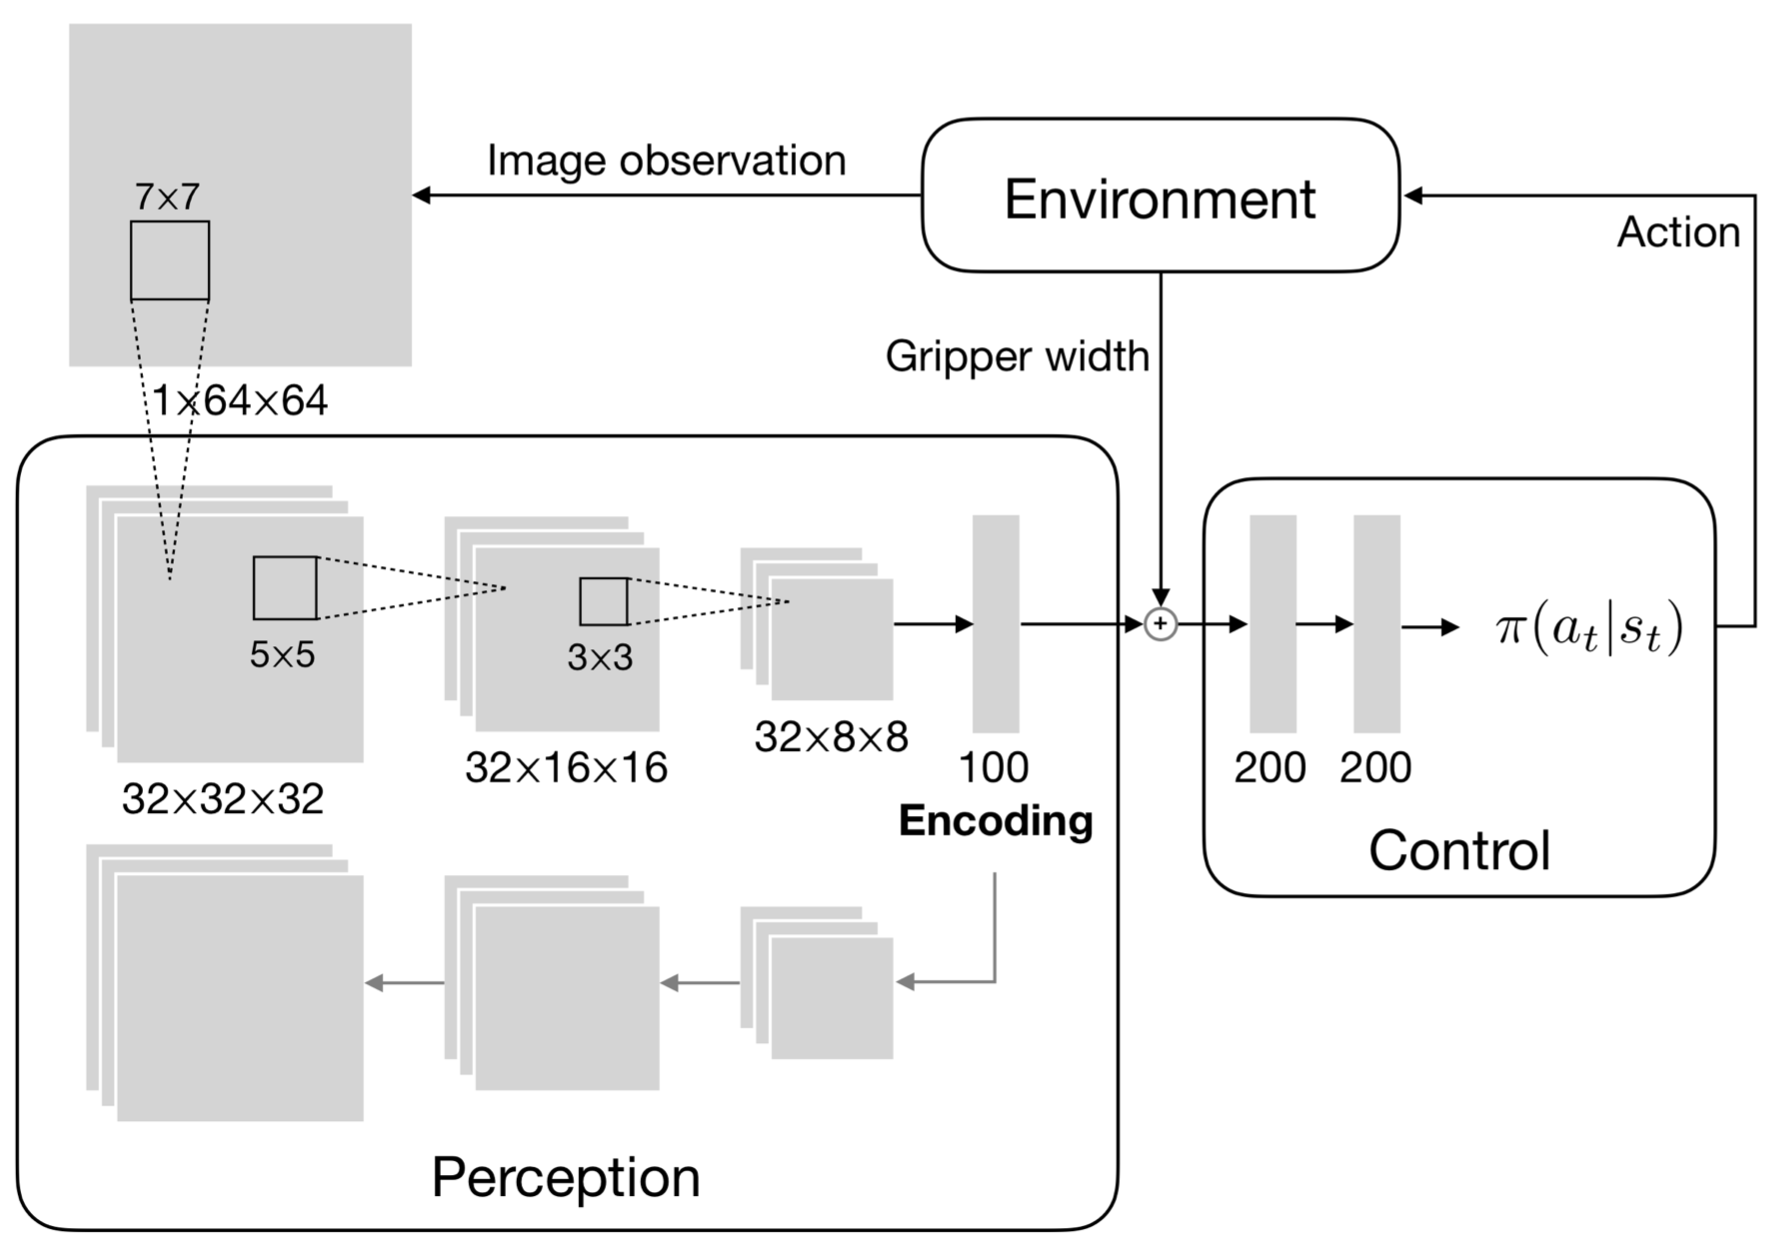
\includegraphics[scale=0.4]{task-simplification}
	\caption{Comparing Task Simplifications to Learn Closed-Loop Object Picking: Network architecture; Source: \cite{tasksimplification}}
	\label{fig:tasksimplification-network}
\end{figure}

\section{Hierarchical reinforcement learning methods}
Traditional reinforcement learning methods are data inefficient (require lot of data for training), difficult to scale (due to large action and/or state space) and brittle due to over specialisation (difficult to transfer their experience to new even similar environments) \cite{gradient}. Hierarchical reinforcement learning are intended to address these issues by learning to operate on different levels of temporal abstraction.

\subsection{Regularized Hierarchical Policies for Compositional Transfer in Robotics}
This method proposes \cite{wulfmeier2019regularized} hierarchical and modular policies for continuous control. The modular hierarchical policy used is defined as:

\begin{equation}
\pi_{\theta} (a | s, i) = \sum_{O=1}^{M} \pi_{\theta}^L(a | s, o) \pi_{\theta}^H(o | s, i)
\end{equation}

Where $\pi^H$ is the high level switching controller and $\pi^L$ is the low level sub policy. The objective is to optimize
\begin{equation}
\underset{q}{max} J(q, \pi_{ref}) = E_{i \sim I} \left[ E_{\pi, s \sim D} \left[ \sum_{t=0}^{\infty} \gamma^t r_i(s_t, a_t) | s_{t+1} \sim p(.|_t, a_t) \right] \right]
\end{equation}
subject to constraint
\begin{equation}
E_{s \sim D, i \sim I} \left[ KL(q(. | s, i) || \pi_{ref}(. | s, i)) \right] \leq \epsilon
\end{equation}

\begin{figure}[H]
	\centering
	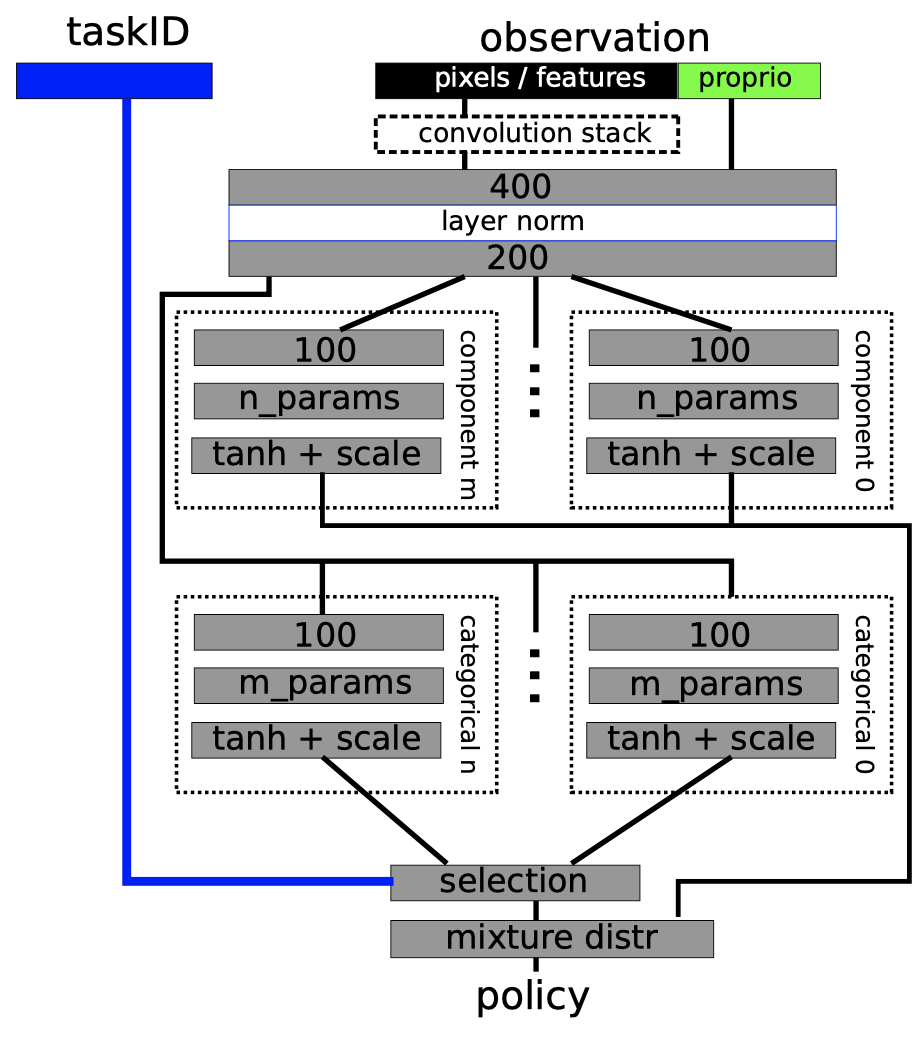
\includegraphics[scale=0.45]{rhpo-arch}
	\caption{RHPO: Network architecture}
\end{figure}